% Original worked example; all graph weights are invented nonnegative integers.
\documentclass[11pt,aspectratio=43]{beamer}
\usetheme{Warsaw}
\usepackage{amsmath,listings,tikz}
\usetikzlibrary{arrows.meta,positioning}
\setbeamertemplate{navigation symbols}{}
\lstset{basicstyle=\ttfamily\small,keywordstyle=\color{blue},columns=fullflexible,keepspaces=true}
\title[Shortest paths]{Find the invariant}
\subtitle{Dijkstra's algorithm, one settled vertex at a time}
\author{Algorithms studio}
\date{Worked example 04}
\begin{document}
\begin{frame}[plain]\titlepage\end{frame}
\begin{frame}{Which path would you try first?}
\centering
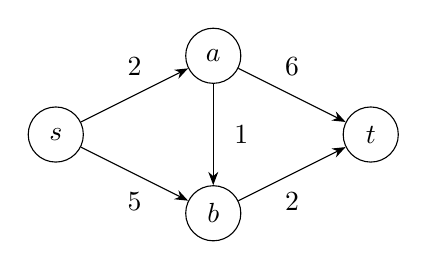
\begin{tikzpicture}[>=Stealth,every node/.style={circle,draw,minimum size=7mm}]
\node (s) at (0,0) {$s$};\node (a) at (2,1) {$a$};
\node (b) at (2,-1) {$b$};\node (t) at (4,0) {$t$};
\draw[->] (s)--node[above,draw=none]{2}(a);
\draw[->] (s)--node[below,draw=none]{5}(b);
\draw[->] (a)--node[right,draw=none]{1}(b);
\draw[->] (a)--node[above,draw=none]{6}(t);
\draw[->] (b)--node[below,draw=none]{2}(t);
\end{tikzpicture}
\medskip
\begin{block}{Prediction}
Before doing arithmetic, identify which tentative distance must become final first.
\end{block}
\end{frame}
\section{Trace the algorithm}
\begin{frame}{The table is the algorithm's working memory}
\begin{center}\begin{tabular}{c|rrrr}
Settled set & $d(s)$ & $d(a)$ & $d(b)$ & $d(t)$\\\hline
$\varnothing$ & $0$ & $\infty$ & $\infty$ & $\infty$\\
\onslide<2->$\{s\}$ & $0$ & $2$ & $5$ & $\infty$\\
\onslide<3->$\{s,a\}$ & $0$ & $2$ & $3$ & $8$\\
\onslide<4->$\{s,a,b\}$ & $0$ & $2$ & $3$ & $5$
\end{tabular}\end{center}\onslide<1->
\only<1>{Initialize one source, not every vertex.}
\only<2>{Relax outgoing edges from $s$.}
\only<3>{The route through $a$ improves $b$.}
\only<4>{The route through $b$ improves the target.}
\end{frame}
\begin{frame}[fragile]{A compact implementation sketch}
\begin{lstlisting}[language=Python]
def shortest_paths(graph, source):
    d = {v: float("inf") for v in graph}
    d[source] = 0
    pending = set(graph)
    while pending:
        u = min(pending, key=lambda v: d[v])
        pending.remove(u)
        for v, w in graph[u]:
            if v in pending:
                d[v] = min(d[v], d[u] + w)
    return d
\end{lstlisting}
\small This simple set-based version scans for the minimum; it is not the heap implementation.
\end{frame}
\section{Explain why}
\begin{frame}{State the claim before proving it}
\begin{theorem}[Settled-distance invariant]
With nonnegative edge weights, each vertex removed with minimum tentative distance has its true shortest-path distance.
\end{theorem}
\pause
\begin{proof}
On a shortest path to the next vertex, consider the first unsettled vertex. Its predecessor was already settled and relaxed that edge. Nonnegative remaining edges prevent the chosen minimum from being too large.
\end{proof}
\end{frame}
\begin{frame}{The assumption is doing real work}
\begin{alertblock}{A counterexample to careless generalization}
Edges $s\to a$ of weight $2$, $s\to b$ of weight $5$, and $b\to a$ of weight $-4$ make $a$ settle too early.
\end{alertblock}
\[
  d_{\mathrm{settled}}(a)=2\qquad\text{but}\qquad\delta(s,a)=1.
\]
No negative cycle is needed for this failure.
\end{frame}
\begin{frame}{Data structure choice changes the cost}
\begin{description}
\item[Scan] Repeated linear minimum selection gives $O(V^2+E)$.
\item[Binary heap] A usual adjacency-list implementation gives $O((V+E)\log V)$.
\item[Unit weights] Breadth-first search avoids the weighted priority queue.
\end{description}
\end{frame}
\section{Practice}
\begin{frame}{Pair exercise: preserve both distance and explanation}
\begin{enumerate}
\item Add predecessor pointers to the sketch.
\item Recover the path $s\to a\to b\to t$.
\item Decide what to return when the target is unreachable.
\item State how ties affect paths and distances differently.
\end{enumerate}
\end{frame}
\begin{frame}{Take the invariant to a new problem}
\begin{block}{One-minute transfer}
Why is ``the first path found'' a valid stopping rule for unweighted BFS, but not for this weighted graph?
\end{block}
\small
\href{https://ocw.mit.edu/courses/6-006-introduction-to-algorithms-fall-2011/resources/mit6_006f11_lec16/}{Reading: MIT 6.006, Lecture 16, Dijkstra.}
\medskip
The graph, trace, pseudocode and exercises in this deck are original.
\end{frame}
\end{document}
